\documentclass[varwidth=true, border=2pt]{standalone}

\usepackage{pgfplots}
\usepackage{tikz}

\begin{document}
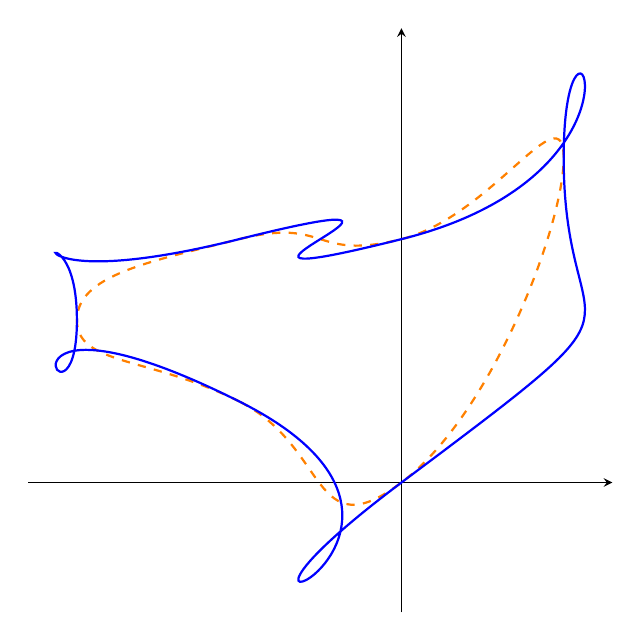
\begin{tikzpicture}
    \begin{axis}[
        legend pos=south west,
        axis x line=middle,
        axis y line=middle,
        %grid = major,
        width=9cm,
        height=9cm,
        grid style={dashed, gray!30},
        xmin=-2,     % start the diagram at this x-coordinate
        xmax= 1,    % end   the diagram at this x-coordinate
        ymin=-1,     % start the diagram at this y-coordinate
        ymax= 5,   % end   the diagram at this y-coordinate
        %axis background/.style={fill=white},
        %xlabel=$x$,
        %ylabel=$y$,
        ticks=none,
        %tick align=outside,
        %minor tick num=-3,
        enlargelimits=true,
        tension=0.08]
        \addplot[mark=none, orange, smooth cycle, thick, tension=1, dashed] coordinates {%
   (0,0) (-1,1) (-2,2) (-1,3) (0, 3) (1, 4)};
        \addplot[mark=none, blue, smooth cycle, thick, tension=3] coordinates {%
   (0,0) (-1,1) (-2,2) (-1,3) (0, 3) (1, 4)};
    \end{axis}
\end{tikzpicture}
\end{document}
